\chapter{Regularization-based Models}
\label{chapter:regularization}

% Shortcut
\newcommand{\mcL}{\mathcal{L}}
\newcommand{\vx}{\mathbf{x}}
\newcommand{\vh}{\mathbf{h}}
\newcommand{\vy}{\mathbf{y}}
\newcommand{\vyh}{\hat\vy}
\newcommand{\pp}{\,\textit{p.p}}


\begin{chapabstract}
    In this chapter, we propose an overview of regularization in Continual Learning. In particular,
    we discuss regularizations that are applied on the networks' outputs and discuss

    The work in this section has led to a publication to a conference paper and a workshop paper:

    \begin{itemize}
        \item \fullcite{douillard2020podnet}
        \item \fullcite{douillard2020ghost}
    \end{itemize}

\end{chapabstract}


\minitoc
\chapterwithfigures{\nameref*{chapter:regularization}}
\chapterwithtables{\nameref*{chapter:regularization}}

\ifthenelse{\boolean{skipRegul}}{\endinput}{}

\section{Introduction}

\ac{CIL}, where each task brings new classes, is among the most challenging setting of \ac{CL}. When
evaluated in single-head, where the task identity is not known at test-time, the majority of the
methods rely on rehearsal learning where a limited amount of old data is replayed. Furthermore, it
is often combined to regularizations that aim to limit forgetting. These regularizations are often a
knowledge distillation \citep{hinton2015knowledge_distillation} that enforces similar probabilities
between the old and current model. First introduced by LwF \citep{li2018lwf}, it has then be used by
multiple seminal papers including iCaRL \citep{rebuffi2017icarl} and WA
\citep{zhao2020weightalignement}. I propose in this chapter two proposed regularization methods to
reduce forgetting. The first one, introduced in \ac{PODNet} \citep{douillard2020podnet}, aims to
regularize the statistics shift at the intermediate feature-level to reduce significantly
catastrophic forgetting. The second one, nicknamed Ghost \citep{douillard2020ghost}, on the other
hand, avoid pre-emptively forgetting by regularizing the feature space at locations where future
classes are estimated to arrive to.

\section{PODNet: reducing forgetting via intermediate feature statistics}

Formally, we learn the model in $T$ \textit{tasks}, task $t$ comprising a set of new classes
$C^t_N$, and a set of old classes $C^t_O$, and aiming at classifying all seen classes $C^t_O \cup
    C^t_N$. Between tasks, the new set $C^t_O$ will be set to $C^{t-1}_O \cup C^{t-1}_N$, but the amount
of training samples from $C^t_O$ (called \textit{memory}) is constrained to exactly $M_\mathrm{per}$
samples per class, while all training samples in the dataset are allowed for the classes in $C^t_N$.

\subsection{Model}
\label{sec:podnet_model}

Our base model is a deep convolutional network $\vyh = g(f(\vx))$, where $\vx$ is the input image,
$\mathbf{y}$ is the output vector of class probabilities, $\vh = f(\vx)$ is the ``feature
extraction'' part of the network (all layers up to the next-to-last), $\vyh = g(\vh)$ is the final
classification layer, and $\vh$ is the final embedding of the network before classification
(\autoref{fig:model}). The superscript $t$ denotes the model learned at task $t$:$f^{t}$, $g^{t}$,
$\vh^{t}$, etc.

Our strategy is made of two keys components: a distillation loss applied at the intermediate
feature-level, and a local-similarity classifier.

\subsubsection{POD: Pooled Outputs Distillation loss}
\label{sec:pod}

Constraining the evolution of the weights is crucial to reduce forgetting. Each new task $t$ learns
a new (student) model, whose weights are not only initialized with those of the previous (teacher)
model, but also constrained by a distillation loss. That loss must be carefully balanced to prevent
forgetting (rigidity), while allowing the learning of new classes (plasticity).

To this goal, we propose a set of constraints we call \textbf{Pooled Outputs Distillation (POD)},
applied not only over the final embedding output by $\vh^{t}=f^{t}(\vx)$, but also over the output
of its intermediate layers $\vh^{t}_\ell=f^{t}_\ell(\vx)$ (where by notation overloading
$f^{t}_\ell(\vx)\equiv f^{t}_\ell\circ\ldots\circ f^{t}_1(\vx)$, and thus $f^{t}(\vx)\equiv
    f^{t}_L\ldots\circ f^{t}_\ell\circ\ldots f^{t}_1(\vx)$).

The convolutional layers of the network output tensors $\vh^{t}_{\ell}$ with components
$\vh^{t}_{\ell,c,w,h}$, where $c$ stands for channel (filter), and $w\times h$ for column and row of
the spatial coordinates. The loss used by POD may pool (sum over) one or several of those indexes,
more aggressive poolings (\autoref{fig:pooling}) providing more freedom, and thus, plasticity: the
lowest possible plasticity imposes an exact similarity between the previous and current model while
higher plasticity relaxes the similarity definition.

Pooling is an important operation in Computer Vision, with a strong theoretical motivation. In the
past, pooling has been introduced to obtain invariant
representations~\citep{lowe1999sift,lazbnik2006spatial_pyramid_matching}. Here, the justification is
similar, but the goal is different: as we will see, the pooled indexes are aggregated in the
proposed loss, allowing \textit{plasticity}. Instead of the model acquiring invariance to the input
image, the desired loss acquires invariance to model evolution, and thus, representation.
%
The proposed pooling-based formalism has two advantages: first, it organizes disparately proposed
distillation losses into a neat, general formalism. Second, as we will see, it allowed us to propose
novel distillation losses, with better plasticity-rigidity compromises. Those topics are explored
next.

\begin{figure}[tb]
    \begin{center}
        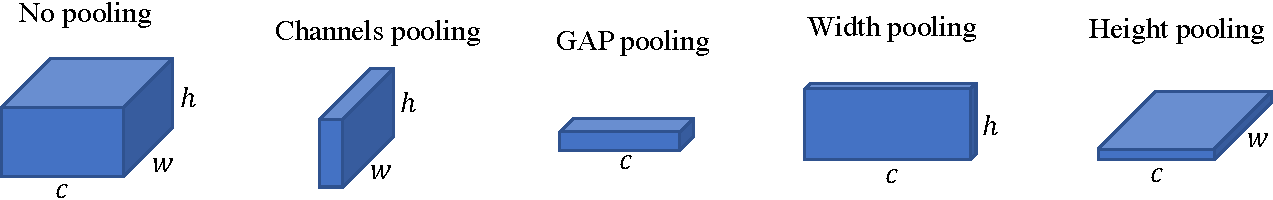
\includegraphics[width=0.90\linewidth]{images/podnet/pooling}
    \end{center}
    \caption{\textbf{Different possible poolings}. The output from a convolutional layer
        $\vh^{t}_{\ell,c,w,h}$ may be pooled (summed over) one or more axes. The resulting loss
        considers only the pooled activations instead of the individual components, allowing more
        plasticity across the pooled axes.}
    \label{fig:pooling}
\end{figure}

\paragraph{Pooling of convolutional outputs} As explained before, POD constrains the output of each
intermediate convolutional layer $\vh^{t}_{\ell,c,w,h} = f^{t}_\ell(\cdot)$ (in practice, each stage
of a ResNet~\citep{he2016resnet}). As a reminder, $c$ is the channel and $w\times h$ are the spatial
coordinates. All POD variants use the Euclidean distance of $\ell^2$-normalize tensors, here noted
as $\left\Vert\cdot-\cdot\right\Vert$. They differ on the type of pooling applied before that
distance is computed.
%
On one extreme, one can apply no pooling at all, resulting in the most strict loss, the most rigid
constrains, and the lowest plasticity:
%
\begin{equation}
    \mcL_{\text{POD-pixel}}(\vh^{t-1}_\ell, \vh^t_\ell) = \sum_{c=1}^C \sum_{w=1}^{W} \sum_{h=1}^{H} \left\Vert \vh^{t-1}_{\ell,c,w,h} - \vh^t_{\ell,c,w,h} \right\Vert^2\label{eq:pod_pixel}\,.
\end{equation}
%
By pooling the channels, one preserves only the spatial coordinates, resulting in a more permissive
loss, allowing the activations to reorganize across the channels, but penalizing global changes of
those activations across the space,
%
\begin{equation}
    \mcL_{\text{POD-channel}}(\vh^{t-1}_\ell, \vh^t_\ell)  = \sum_{w=1}^{W} \sum_{h=1}^{H} \left\Vert \sum_{c=1}^C \vh^{t-1}_{\ell,c,w,h} - \sum_{c=1}^C \vh^{t}_{\ell,c,w,h} \right\Vert^2\label{eq:pod_channel}\,;
\end{equation}
%
or, contrarily, by pooling the space (equivalent, up to a factor, to a Global Average Pooling), one
preserves \textit{only} the channels:
%
\begin{equation}
    \mcL_{\text{POD-gap}}(\vh^{t-1}_\ell, \vh^t_\ell) = \sum_{c=1}^{C} \left\Vert \sum_{w=1}^{W} \sum_{h=1}^H \vh^{t-1}_{\ell,c,w,h} - \sum_{w=1}^{W} \sum_{h=1}^H \vh^{t}_{\ell,c,w,h} \right\Vert^2\label{eq:pod_gap}\,.
\end{equation}
%

Note that the only difference between the variants is in the position of the summation. For example,
contrast equations \autoref{eq:pod_pixel} and \ref{eq:pod_channel}: in the former the differences
are computed between activation pixels, and then totaled; in the latter, first the channel axis is
flattened, then the differences are computed, resulting in a more permissive loss.

We can trade a little plasticity for rigidity, with less aggressive pooling by aggregating
statistics across just one of the spatial dimensions:
%
\begin{equation}
    \mcL_{\text{POD-width}}(\vh^{t-1}_\ell, \vh^t_\ell)  = \sum_{c=1}^{C} \sum_{h=1}^{H} \left\Vert \sum_{w=1}^W \vh^{t-1}_{\ell,c,w,h} - \sum_{w=1}^W \vh^{t}_{\ell,c,w,h} \right\Vert^2\label{eq:pod_width}\,;
\end{equation}
%
or, likewise, for the vertical dimension, resulting in POD-height. Each of those variants measure
the distribution of activation pixels across their respective axis. These two complementary
intermediate statistics can be further combined together:
%
\begin{equation}
    \mcL_{\text{POD-spatial}}(\vh^{t-1}_\ell, \vh^t_\ell) = \mcL_{\text{POD-width}}(\vh^{t-1}_\ell, \vh^t_\ell) + \mcL_{\text{POD-height}}(\vh^{t-1}_\ell, \vh^t_\ell)\,.
\end{equation}
%
$\mcL_{\text{POD-spatial}}$ is minimal when the average statistics over the dataset, on both width
and height axes, are similar for the previous and current model. It brings the right balance between
being too rigid (\autoref{eq:pod_pixel}) and being too permissive (\autoref{eq:pod_channel} and
\ref{eq:pod_gap}).

\label{sec:pod_flat}
\paragraph{Constraining the final embedding} After the convolutional layers, the network, by design,
flattens the spatial coordinates, and the formalism above needs adjustment, as a summation over $w$
and $h$ is no longer possible. Instead, we set a flat constraint on the final embedding $\vh^{t} =
    f^{t}(\vx)$:
%
\begin{equation}
    \mcL_{\text{POD-flat}}(\vh^{t-1}, \vh^t) = \left\Vert \vh^{t-1} - \vh^t \right\Vert^2\label{eq:POD-flat}\,.
\end{equation}

\paragraph{Combining the losses, analysis} The final POD loss combines the two  components:
%
\begin{multline}
    \mcL_\text{POD-final}(\vx) =  \frac{\lambda_{c}}{L-1}\sum_{\ell=1}^{L-1}  \mcL_{\text{POD-spatial}}\left(f^{t-1}_\ell(\vx), f^t_\ell(\vx)\right) + \\[-0.8em]
    \lambda_{f} \mcL_\text{POD-flat}\left(f^{t-1}(\vx), f^t(\vx)\right)\,.
\end{multline}
%
The hyperparameters $\lambda_{c}$ and $\lambda_{f}$ are necessary to balance the two terms, due to
the  different nature of the intermediate outputs (spatial and flat).

As mentioned, the strategy above generalizes disparate propositions existing both in the literature
of incremental learning, and elsewhere. When $\lambda_{c}=0$, it reduces to the cosine constraint of
\textit{Less-Forget}, proposed by Hou et al. for incremental learning, which constrains only the
final embedding~\citep{hou2019ucir}. When $\lambda_{f}=0$ and POD-spatial is replaced by POD-pixel,
it suggests the Perceptual Features loss, proposed for style
transfer~\citep{johnson2016perceptual_losses}. When $\lambda_{f}=0$ and POD-spatial is replaced by
POD-channel, the strategy hints at the loss proposed by Komodakis et
al.~\citep{komodakis2017attention_residual_distillation} to allow distillation across different
networks, a situation in which the channel pooling responds to the very practical need to allow the
comparison of architectures with different number of channels.

As we will see in our evaluations of pooling strategies (\autoref{sec:ablation_pooling}), what
proved optimal was a completely novel idea, POD-spatial, combining two poolings, each of which
flattens one of the spatial coordinates. That relatively rigid strategy (channels and one of the
spatial coordinates are considered in each half of the loss) makes intuitive sense in our context,
which is \textit{small-task} incremental learning, and thus where we expect a slow drift of the
model across a single task.

% ------------------------------------------------------------

\begin{figure}[t]
    \begin{center}
        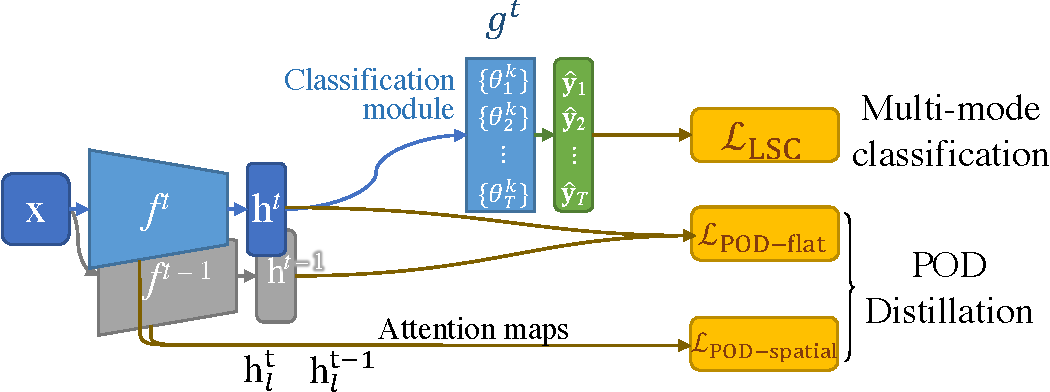
\includegraphics[width=0.8\linewidth]{images/podnet/model}
    \end{center}
    \caption{\textbf{Overview of PODNet}: the distillation loss POD prevent excessive model drift by
        constraining intermediate outputs of the ConvNet $f$ and the LSC classifier $g$ learns a
        more expressive multi-modal representation.}
    \label{fig:model}
\end{figure}

\subsubsection{Local Similarity Classifier}
\label{sec:local_classifier}

Hou et al.~\citep{hou2019ucir} observed that the class imbalance of incremental learning have
concrete manifestations on the parameters of the final layer on classifiers, namely the weights for
the over-represented (new) classes becoming much larger than those for the underrepresented (old)
classes. To overcome this issue, their method (called here UCIR) $\ell^2$-normalizes both the
weights and the activations, which corresponds to taking the cosine similarity instead of the dot
product. For each class $c$, their last layer becomes
%
\begin{equation}
    \vyh_{c}=\frac{\exp\left(\eta\langle\theta_{c},\vh\rangle\right)}{\sum_{i} \exp \left(\eta\langle\theta_{i}, \vh\rangle\right)}\,,
\end{equation}
%
where $\theta_c$ are the last-layer weights for class $c$, $\eta$ is a learned scaling parameter,
and $\langle\cdot,\cdot\rangle$ is the cosine similarity.

However, this strategy optimizes a \textit{global similarity}: its training objective increases the
similarity between the extracted features and their associated weights. For each class, the
normalized weight vector acts as a \textit{single} proxy~\citep{attias2017proxynca}, towards which
the learning procedure pushes all samples in the class.

We observed that such global strategy is hard to optimize in an incremental setting. To avoid
forgetting, the distillation losses (\autoref{sec:distillation}) tries to keep the final embedding
$\vh$ consistent through time so that the class proxies stay relevant for the classifier.
Unfortunately catastrophic forgetting, while alleviated by current methods, is not solved and thus
the distribution of $\vh$ may change. The cosine classifier is very sensitive to those changes as it
models a unique majority mode through its class proxies.


\paragraph{Local Similarity Classifier} The problem above lead us to amend the classification layer
during training, in order to consider multiple proxies/modes per class. A shift in the distribution
of $\vh$ will have less impact on the classifier as more modes are covered.


Our redesigned classification layer, which we call Local Similarity Classifier (LSC), allows for $K$
multiple proxies/modes during training. Like before, the proxies are a way to interpret the weight
vector in the cosine similarity, thus we allow for $K$ vectors $\theta_{c,k}$ for each class $c$.
The similarity $s_{c,k}$ to each proxy/mode is first computed. An averaged class similarity $\vyh_c$
is the output of the classification layer:
%
\begin{equation}
    s_{c,k} =\frac{\exp\,\langle\theta_{c,k},\vh\rangle}{\sum_{i} \exp\,\langle\theta_{c,i},\vh\rangle}\,, \qquad
    \vyh_c = \sum_{k}s_{c,k}\,\langle\theta_{c,k},\vh\rangle\,.
\end{equation}
%
The multi-proxies classifier optimizes the similarity of each sample to its ground truth class
representation and minimizes all others. A simple cross-entropy loss would work, but we found
empirically that the NCA loss~\citep{goldberger2005nca_loss,attias2017proxynca} converged faster. We
added to the original loss a hinge $[\,\cdot\,]_+$ to keep it bounded, and a small margin $\delta$
to enforce stronger class separation, resulting in the final formulation:
%
\begin{equation}
    \mcL_\text{LSC} = \left[- \log\frac{\exp\left(\eta (\vyh_y - \delta)\right)}{\sum_{i \neq y} \exp \eta \vyh_{i}} \right]_+ \,.
\end{equation}

\paragraph{Weight initialization for new classes} The incremental learning setting imposes detecting
new classes at each new task $t$. New weights $\{\theta_{c,k} \mid \forall c \in C^t_N, \forall k
    \in {1...K}\}$ must be added to predict them. We could initialize them randomly, but the
class-agnostic features of the ConvNet $f$, extracted by the model trained so far offer a better
prior. Thus, we employ a generalization of Imprinted Weights~\citep{qi2018imprintedweights}
procedure to multiple modes: for each new class $c$, we extract the features of its training
samples, use a k-means algorithm to split them into $K$ clusters, and use the centroids of those
clusters as initial values for $\theta_{c,k}$. This procedure ensures mode diversity at the
beginning of a new task and resulted in a one percentage point improvement on CIFAR100.

% ------------------------------------------------------------

\subsubsection{Complete model formulation}

Our model has the classical structure of a convolutional network $f(\cdot)$ acting as a feature
extractor, and a classifier $g(\cdot)$ producing a score per class. We introduced two innovations to
this model: (1) our main contribution is a novel distillation loss (POD) applied all over the
ConvNet, from the spatial features $\vh_\ell$ to the final flat embedding $\vh$; (2) as further
refinement we propose that the classifier learns a multi-modal representation that explicitly keeps
multiple proxy vectors per class, increasing the model expressiveness and thus making it less
sensible to shift in the distribution of $\vh$. The final loss for current model $g^t \circ f^t$,
i.e., the model trained for task $t$, is simply their addition $\mathcal{L}_{\{f^t; g^t\}} =
    \mathcal{L}_\textrm{LSC} + \mathcal{L}_\textrm{POD-final}$.

\subsection{Experiment results}


We compare our technique (PODNet) with three state-of-the-art models. Those models are particularly
comparable to ours since they all employ a sample memory with a fixed capacity. Both
iCaRL~\citep{rebuffi2017icarl} and UCIR~\citep{hou2019ucir} use the same inference method
--\,\textit{Nearest-Mean-Examplars} (NME), although UCIR also proposes a second inference method
based on the classifier probabilities (called here UCIR-CNN). We evaluate PODNet with both inference
methods for a small scale dataset, and the later for larger scale datasets.
BiC~\citep{wu2019bias_correction}, while not focused on representation learning, is specially
designed to be effective on large scale datasets, and thus provided an interesting baseline.

\paragraph{Datasets} We employ three images datasets --\,extensively used in the literature of
incremental learning\,-- for our experiments: CIFAR100~\citep{krizhevskycifar100},
ImageNet100~\citep{deng2009imagenet,hou2019ucir,wu2019bias_correction}, and
ImageNet1000~\citep{deng2009imagenet}. ImageNet100 is a subset of ImageNet1000 with only 100
classes, randomly sampled from the original 1000.

{\begin{description} \setlength{\parskip}{0pt}
    \item[CIFAR100] contains 32$\times$32-pixel images in 100 classes, with 50k images for training
          and 10k for testing.
    \item[ImageNet100] contains 224$\times$224-pixel images in 100 classes, with $\sim$128k images
          for training and $\sim$5k for testing.
    \item[ImageNet1000] contains 224$\times$224-pixel images in 1000 classes, with $\sim$1.28m
          images for training and $\sim$50k for testing.
\end{description}}

\paragraph{Protocol} We validate our model and the compared baselines using the challenging protocol
introduced by Hou et al.~\citep{hou2019ucir}: we start by training the models on half the classes
(i.e., 50 for CIFAR100 and ImageNet100, and 500 for ImageNet1000). Then the classes are added
incrementally in steps. We divide the remaining classes equally among the steps, e.g., for CIFAR100
we could have 5 steps of 10 classes or 50 steps of 1 class. Note that a training of 50 steps is
actually made of 51 different tasks: the initial training followed by the incremental steps. Models
are evaluated after each step on \textit{all the classes seen until then}. To facilitate comparison,
the accuracies at the end of each step are averaged into a unique score called \textit{average
    incremental accuracy}~\citep{rebuffi2017icarl}. If not specified otherwise, the average incremental
accuracy is the score reported in all our results.

%For CIFAR100, we ran all experiments thrice, varying the order of the classes. We report the
%averages and standard deviations in tables and graphs. For ImageNet100 and ImageNet1000, whose
%models took much longer to train, we ran each experiment once.

Following Hou et al.~\citep{hou2019ucir}, for all datasets, and all compared models, we limit the
memory $M_\textrm{per}$ to 20 images per old class. For results with different memory settings,
refer to \autoref{sec:robustness}.

\paragraph{Implementation details} For fair comparison, all compared models employ the same ConvNet
backbone: ResNet-32 for CIFAR100, and ResNet-18 for ImageNet. We remove the ReLU activation at the
last block of each ResNet end-of-stage to provide a signed input to POD
(\autoref{sec:distillation}). We implemented our method (called here PODNet) in
PyTorch~\citep{paszke2017pytorch}.
%
We compare both ours and UCIR's implementation~\citep{hou2019ucir} of iCaRL. Results of UCIR come
from the implementation of Hou et al.~\citep{hou2019ucir}. We provide their reported results and
also run their code ourselves. We used our implementation of BiC in order to compare with the same
backbone.
%
We sample our memory images using \textit{herding selection}~\citep{rebuffi2017icarl} and perform
the inference with two different methods: the \textit{Nearest-Mean-Examplars} (NME) proposed for
iCarl, and also adopted on one of the variants of UCIR~\citep{hou2019ucir}, and the ``CNN'' method
introduced for UCIR (see \autoref{sec:related_work}).
%
Please see the supplementary materials for the full implementation details.

\begin{table*}[t]
    \centering
    \begin{adjustbox}{max width=\textwidth}
        \begin{tabular}{@{}l|cccc@{}}
            \toprule
                                                                         & \multicolumn{4}{|c}{CIFAR100}                                                                            \\
                                                                         & 50 steps                      & 25 steps               & 10 steps               & 5 steps                \\
            \multicolumn{1}{r|}{New classes per step}                    & 1                             & 2                      & 5                      & 10                     \\
            \midrule
            \textit{iCaRL*} \citep{rebuffi2017icarl}                     & ---                           & ---                    & 52.57$\mspace{51mu}$   & 57.17$\mspace{51mu}$   \\
            iCaRL                                                        & 44.20\std0.98                 & 50.60\std1.06          & 53.78\std1.16          & 58.08\std0.59          \\
            BiC \citep{wu2019bias_correction}                            & 47.09\std1.48                 & 48.96\std1.03          & 53.21\std1.01          & 56.86\std0.46          \\
            \textit{UCIR\,{\scriptsize (\ac{NME})}*} \citep{hou2019ucir} & ---                           & ---                    & 60.12$\mspace{51mu}$   & 63.12$\mspace{51mu}$   \\
            UCIR\,{\scriptsize (\ac{NME})}                               & 48.57\std0.37                 & 56.82\std0.19          & 60.83\std0.70          & 63.63\std0.87          \\
            \textit{UCIR\,{\scriptsize (CNN)}*}                          & ---                           & ---                    & 60.18$\mspace{51mu}$   & 63.42$\mspace{51mu}$   \\
            UCIR\,{\scriptsize (CNN)}                                    & 49.30\std0.32                 & 57.57\std0.23          & 61.22\std0.69          & 64.01\std0.91          \\
            PODNet\,{\scriptsize (\ac{NME})}                             & \textbf{61.40\std0.68}        & \textbf{62.71\std1.26} & \textbf{64.03\std1.30} & \textbf{64.48\std1.32} \\
            PODNet\,{\scriptsize (CNN)}                                  & \textbf{57.98\std0.46}        & \textbf{60.72\std1.36} & \textbf{63.19\std1.16} & \textbf{64.83\std0.98} \\
            \bottomrule
        \end{tabular}
    \end{adjustbox}
    \caption{\textbf{CIFAR100 quantitative experiments:} Average incremental accuracy for PODNet \vs state of the art. We run
        experiments three times (random class orders) on CIFAR100 and report averages and
        standard deviations. Models with an asterisk * are reported directly from
        \cite{hou2019ucir}}
    \label{tab:podnet_quantitative_cifar}
\end{table*}

\begin{table*}[t]
    \centering
    \begin{adjustbox}{max width=\textwidth}
        \begin{tabular}{@{}l|cccc|cc@{}}
            \toprule
                                                                             & \multicolumn{4}{|c|}{ImageNet100} & \multicolumn{2}{c}{Imagenet1000}                                                                                                         \\
            %\cmidrule(l{0pt}r{4pt}){2-4} \cmidrule(l{4pt}r{4pt}){5-7} \cmidrule(l{4pt}r{4pt}){8-9}
                                                                             & 50 steps                          & 25 steps                         & 10 steps                         & 5 steps                          & 10 steps       & 5 steps        \\
            \multicolumn{1}{r|}{New classes per step}                        & 1                                 & 2                                & 5                                & 10                               & 50             & 100            \\
            \midrule
            iCaRL* \scriptsize{\citep{rebuffi2017icarl}}                     & ---                               & ---                              & 59.53                            & 65.04                            & 46.72          & 51.36          \\
            iCaRL                                                            & 54.97                             & 54.56                            & 60.90                            & 65.56                            & ---            & ---            \\
            BiC \scriptsize{\citep{wu2019bias_correction}}                   & 46.49                             & 59.65                            & 65.14                            & 68.97                            & 44.31          & 45.72          \\
            UCIR\,{\scriptsize (\ac{NME})}* \scriptsize{\citep{hou2019ucir}} & ---                               & ---                              & 66.16                            & 68.43                            & 59.92          & 61.56          \\
            UCIR\,{\scriptsize (\ac{NME})}                                   & 55.44                             & 60.81                            & 65.83                            & 69.07                            & ---            & ---            \\
            UCIR\,{\scriptsize (CNN)}*                                       & ---                               & ---                              & 68.09                            & 70.47                            & 61.28          & 64.34          \\
            UCIR\,{\scriptsize (CNN)}                                        & 57.25                             & 62.94                            & 67.82                            & 71.04                            & ---            & ---            \\
            % PODNet\,{\scriptsize (CNN)}                & \textbf{62.48 $\pm$ 0.59} & \textbf{68.31 $\pm$ 2.45} & \textbf{74.33 $\pm$ 0.93} & \textbf{75.54 $\pm$ 0.26} & \textbf{64.13} & \textbf{66.95}\\
            PODNet\,{\scriptsize (CNN)}                                      & \textbf{62.48}                    & \textbf{68.31}                   & \textbf{74.33}                   & \textbf{75.54}                   & \textbf{64.13} & \textbf{66.95} \\

                                                                             & \scriptsize{\textbf{$\pm$ 0.59}}  & \scriptsize{\textbf{$\pm$ 2.45}} & \scriptsize{\textbf{$\pm$ 0.93}} & \scriptsize{\textbf{$\pm$ 0.26}} &                &                \\

            \bottomrule
        \end{tabular}
    \end{adjustbox}
    \caption{\textbf{ImageNet quantitative experiments:} Average incremental accuracy, PODNet \vs
        state of the art. Models with an asterisk * are reported directly from \citet{hou2019ucir}.
        The initial task's sizes are respectively 50 and 500 classes for ImageNet100 and
        ImageNet1000. The remaining classes are learned incrementally.}
    \label{tab:podnet_quantitative_imagenet}
\end{table*}


\subsection{Quantitative results}
\label{sec:quantitative_results}

The comparisons with all the state of the art are tabulated in \autoref{tab:quantitative_cifar} for
CIFAR100 and \autoref{tab:quantitative_imagenet} for ImageNet100 and ImageNet1000. All tables shows
the average incremental accuracy for each considered models with various number of steps on the
incremental learning run. The ``New classes per step'' row shows the amount of new classes
introduced per task.

\paragraph{CIFAR100} We run our comparisons on 5, 10, 25, and 50 steps with respectively 10, 5, 2,
and 1 classes per step. We created three random class orders to ran each experiment thrice,
reporting averages and standard deviations. For CIFAR100 only, we evaluated our model with two
different kind of inference: NME and CNN. With both methods, our model surpasses all previous state
of the art models on all steps. Moreover, our model relative improvement grows as the number the
steps increases, surpassing existing models by 0.82, 2.81, 5.14, and 12.1 percent points (\pp) for
respectively 5, 10, 25, and 50 steps. Larger numbers of steps imply  stronger forgetting; those
results confirm that PODNet manages to reduce drastically the said forgetting. While PODNet with NME
has the largest gain, PODNet with CNN also outperforms the previous state of the art by up to
8.68\pp. See \autoref{fig:plots} for a plot of the incremental accuracies on this dataset. In the
extreme setting of 50 increments of 1 class (\autoref{fig:cifar_inc1}), our model showcases large
differences, with slow degradation (``\textit{gradual forgetting}''
\citep{french1999catastrophicforgetting}) due to forgetting throughout the run, while the other
models show a quick performance collapse (``\textit{catastrophic forgetting}'') at the start of the
run.

\paragraph{ImageNet100} We run our comparisons on 5, 10, 25, and 50 steps with respectively 10, 5,
2, and 1 classes per step. For both ImageNet100, and ImageNet1000 we report only PODNet with CNN, as
the kNN-based NME classifier did not generalize as well to larger-scale datasets. With the more
complex images of ImageNet100, our model also outperforms the state of the art on all tested runs,
by up to 6.51\pp.

\paragraph{ImageNet1000} This dataset is the most challenging, with much greater image complexity
than CIFAR100, and ten times the number of classes as ImageNet100. We evaluate the models in 5 and
10 steps, and results confirm the consistent improvement of PODNet against existing arts by up to
2.85\pp.

\begin{table*}
    \centering
    \begin{tabular}{@{}lccccc@{}}
        \toprule
        Classifier & POD-flat & POD-spatial & NME            & CNN            \\
        \midrule
        Cosine     &          &             & 40.76          & 37.93          \\
        Cosine     & \OK      &             & 48.03          & 46.73          \\
        Cosine     &          & \OK         & 54.32          & 57.27          \\
        Cosine     & \OK      & \OK         & 56.69          & 55.72          \\
        LSC-CE     & \OK      & \OK         & 59.86          & 57.45          \\
        LSC        &          &             & 41.56          & 40.76          \\
        LSC        & \OK      &             & 53.29          & 52.98          \\
        LSC        &          & \OK         & \textbf{61.42} & 57.64          \\
        LSC        & \OK      & \OK         & 61.40          & \textbf{57.98} \\
        \bottomrule
    \end{tabular}
    \caption{Comparison of the average incremental accuracy on CIFAR100 with 50 steps of the model when disabling parts of the complete \ac{PODNet} loss\\~}
    \label{tab:podnet_ablation_inc}
\end{table*}

\begin{figure*}[tb]
    \centering
    \begin{subfigure}[b]{0.48\linewidth}
        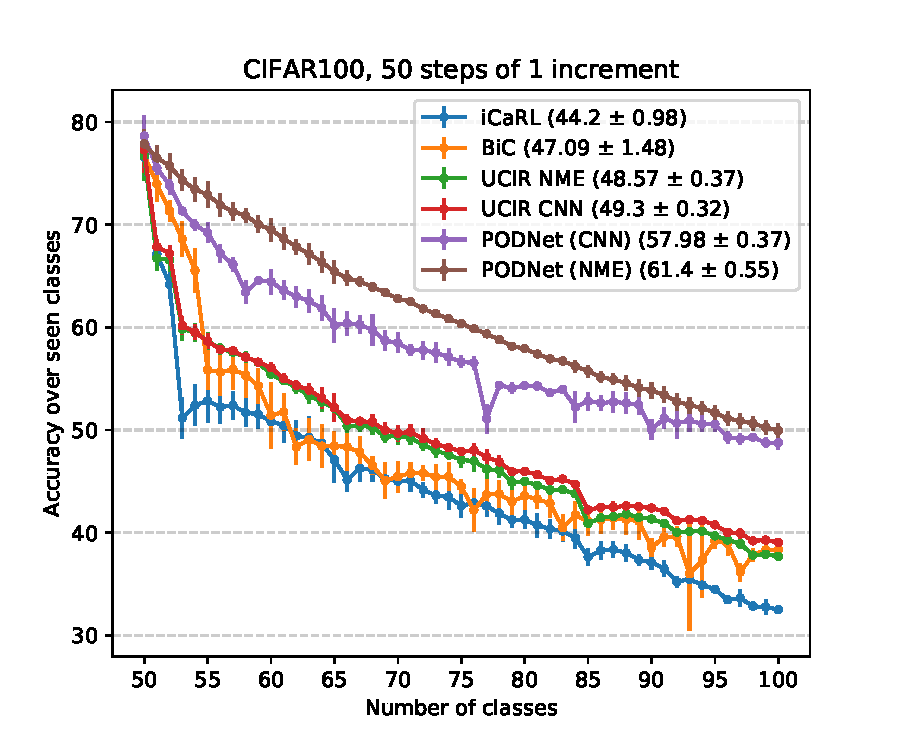
\includegraphics[width=\linewidth]{images/podnet/cifar_inc1}
        \caption{50 steps, 1 class / step}
        \label{fig:cifar_inc1}
    \end{subfigure}
    \hfill
    \begin{subfigure}[b]{0.48\linewidth}
        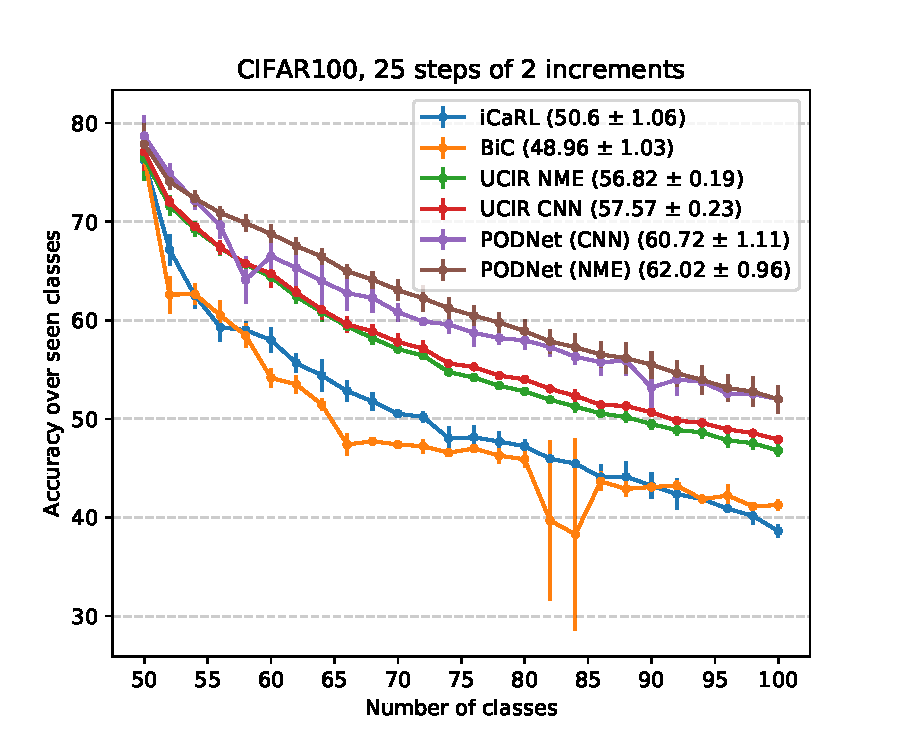
\includegraphics[width=\linewidth]{images/podnet/cifar_inc2}
        \caption{25 steps, 2 classes / step}
        \label{fig:cifar_inc2}
    \end{subfigure}
    \caption{\textbf{Incremental Accuracy on CIFAR100} over three orders for two different step sizes. The legend reports the average incremental accuracy.}
    \label{fig:plots}
\end{figure*}


\subsection{Further analysis \& ablation studies}
\label{sec:ablation}

\paragraph{Ablation Studies}
Our model has two components: the distillation loss POD and the LSC classifier. An ablation study
showcasing the contribution of each component is displayed in \autoref{tab:ablation_inc}: each
additional component improves the model performance. We evaluate every ablation on CIFAR100 with 50
steps of 1 new class each. The reported metric is the average incremental accuracy. The table shows
that our novel method of constraining the whole ConvNet is beneficial. Furthermore applying only
POD-spatial still beats the previous state of the art by a significant margin. Using both
POD-spatial and POD-flat then further increases results with a large gain. We also compare the
results with the Cosine classifier~\citep{luo2018cosine_classifier,hou2019ucir} against the Local
Similarity Classifier (LSC) with NCA loss. Finally, we add LSC-CE: our classifier with multi-mode
but with a simple cross-entropy loss instead of our modified NCA loss. This version brings to mind
SoftTriple~\citep{qian2019softtriple} and Infinited Mixture
Prototypes~\citep{allen2019infinitemixtureproto}, used in the different context of few-shot
learning.
%The former adds a regularization loss to collapse the multiple proxies into a single one if
%necessary, which we did not find useful in our imbalanced setting of incremental learning.
The latter only considers the closest mode of each class in its class assignment, while LSC
considers all modes of a class, thus, taking into account the intra-class variance. That allows LSC
to decrease class similarity when intra-class variance is high (which could signal a lack of
confidence in the class).

\label{sec:ablation_pooling}
\paragraph{Spatial-based distillation} We apply our distillation loss POD differently for the flat
final embedding $\vh$ (POD-flat) and the ConvNet's intermediate features maps $\vh_\ell$
(POD-spatial). We designed and evaluated several alternative for the latter whose results are shown
in \autoref{tab:ablation_perceptual}. Refer to \autoref{sec:distillation} and \autoref{fig:pooling}
for their definition. All losses are evaluated with POD-flat. "\textit{None}" is using only
POD-flat.
%POD-pixels (\ref{eq:pod_pixel}) doesn't pool the features maps and is simply an euclidean distance
%pixel-wise for all channels. POD-gap does a \textit{global average pooling} over spatial dimension.
%POD-channels sum-pools the channels axis. POD-width and POD-height sum-pools respectively the
%horinzontal and vertical axis. Finally POD-spatial is the union of both POD-width and POD-height.
Overall, we see that not using pooling results in bad performance (POD-pixels). Our final loss,
POD-spatial, surpasses all others by taking advantages of the statistics aggregated from both
spatial axis. For the sake of completness we also included losses not designed by us: GradCam
distillation~\citep{dhar2019learning_without_memorizing_gradcam} and Perceptual
Style~\citep{johnson2016perceptual_losses}. The former uses a gradient-based attention while the
later --\,used for style transfer\,-- computes a gram matrix for each channel.

\paragraph{Forgetting and plasticity balance} Forgetting can be drastically reduced by imposing a
high factor on the distillation losses. Unfortunately, it will also degrade the capacity (its
\textit{plasticity}) to learn new classes. When POD-spatial is added on top of POD-flat, we manage
to increase the oldest classes performance (+7 percentage points) while the newest classes
performance were barely reduced (-0.2\pp). Because our loss POD-spatial constraints only statistics,
it is less stringent than a loss based on exact pixels values as POD-pixel. The latter hurts the
newest classes (-2\pp) for a smaller improvement of old classes (+5\pp). Furthermore our experiments
confirmed that LSC reduced the sensibility of the model to distribution shift, as the performance it
brings was localized on the old classes.

\label{sec:robustness}
\paragraph{Robustness of our model} While previous results showed that PODNet improved significantly
over the state-of-the-arts, we wish here to demonstrate here the robustness of our model to various
factors. In \autoref{tab:ablation_memorysize}, we compared how PODNet behaves against the baseline
when the memory size per class $M_{\text{per}}$ changes: PODNet improvements increase as the memory
size decrease, up to a gain of 26.20\pp\ with NME (resp. 13.42\pp\ for CNN) with $M_{\text{per}} =
    5$. Notice that by default, the memory size is 20 in \autoref{sec:quantitative_results}.
% We also compared our model against baselines with a $M_{\text{total}} = 2000$ in
% \autoref{tab:sub_free_memory}, and with various initial task size (by default it is 50 on
% CIFAR100) in \autoref{tab:sub_initialincrement}. In the former case, models benefit from a larger
% memory per class in the early tasks. In the later case, models initialization is worse with
% smaller initial task size. In these settings very different from
% \autoref{sec:quantitative_results}, PODNet still outperformed significantly the compared models,
% proving the robustness of our model.
We also compared our model against baselines with a more flexible memory $M_{\text{total}} = 2000$
\citep{rebuffi2017icarl,wu2019bias_correction}, and with various initial task size (by default it is
50 on CIFAR100). In the former case (\autoref{tab:sub_free_memory}), models benefit from a larger
memory per class in the early tasks. In the later case (\autoref{tab:sub_initialincrement}), models
initialization is worse because of a smaller initial task size. In these settings very different
from \autoref{sec:quantitative_results}, PODNet still outperformed significantly the compared
models, proving the robustness of our model.

\begin{table}[t]
    \centering
    \begin{tabular}{@{}lccccccc@{}}
        \toprule
        $M_{per}$                                                       & 5              & 10             & \textbf{20}    & 50             & 100            & 200            \\
        \midrule
        iCaRL \scriptsize{\citep{rebuffi2017icarl}}                     & 16.44          & 28.57          & 44.20          & 48.29          & 54.10          & 57.82          \\
        BiC \scriptsize{\citep{wu2019bias_correction}}                  & 20.84          & 21.97          & 47.09          & 55.01          & 62.23          & \textbf{67.47} \\
        UCIR\,{\scriptsize (\ac{NME})} \scriptsize{\citep{hou2019ucir}} & 21.81          & 41.92          & 48.57          & 56.09          & 60.31          & 64.24          \\
        UCIR\,{\scriptsize (CNN)}                                       & 22.17          & 42.70          & 49.30          & 57.02          & 61.37          & 65.99          \\
        PODNet\,{\scriptsize (\ac{NME})}                                & \textbf{48.37} & \textbf{57.20} & \textbf{61.40} & \textbf{62.27} & \textbf{63.14} & 63.63          \\
        PODNet\,{\scriptsize (CNN)}                                     & \textbf{35.59} & \textbf{48.54} & \textbf{57.98} & \textbf{63.69} & \textbf{66.48} & \textbf{67.62} \\
        \bottomrule
    \end{tabular}
    \caption{\textbf{Effect of the memory size} per class $M_{per}$ on the models performance.
        Results from CIFAR100 with 50 steps, we report the average incremental accuracy}
    \label{tab:podnet_ablation_memorysize}
\end{table}

\captionsetup[table]{skip=0pt}
\begin{table}[t]
    \setlength{\tabcolsep}{2.7pt}
    \caption{Effect of the initial task size and the $M_\mathrm{total}$ on the models performance. We report the average incremental accuracy}
    \begin{subtable}[b]{.36\textwidth}
        \centering
        \caption{Evaluation of an easier memory constraint ($M_\mathrm{total} = 2000$)}
        \label{tab:sub_free_memory}
        \begin{tabular}{@{}lcc@{}}
            \toprule
                                                          & \multicolumn{2}{c}{Nb. steps}                  \\
            \cmidrule{2-3}
            Loss                                          & 50                            & 10             \\
            \midrule
            iCaRL \cite{rebuffi2017icarl}                 & 42.34                         & 56.52          \\
            BiC \cite{wu2019bias_correction}              & 48.44                         & 55.03          \\
            UCIR\,{\scriptsize (NME)}\,\cite{hou2019ucir} & 54.08                         & 62.89          \\
            UCIR\,{\scriptsize (CNN)}\,\cite{hou2019ucir} & 55.20                         & 63.62          \\
            PODNet\,{\scriptsize (NME)}                   & \textbf{62.47}                & \textbf{64.60} \\
            PODNet\,{\scriptsize (CNN)}                   & \textbf{61.87}                & \textbf{64.68} \\
            \bottomrule
        \end{tabular}
    \end{subtable}
    %
    \hfill
    %
    \begin{subtable}[b]{.62\textwidth}
        \centering
        \caption{Varying initial task size, with $M_\mathrm{per} = 20$, and followed by 50 to 90 tasks made of a single class}
        \label{tab:sub_initialincrement}
        \begin{tabular}{@{}lccccc@{}}
            \toprule
                                                         & \multicolumn{5}{c}{Initial task size}                                                                     \\
            \cmidrule{2-6}
            Loss                                         & 10                                    & 20             & 30             & 40             & \textbf{50}    \\
            \midrule
            iCaRL \cite{rebuffi2017icarl}                & 40.97                                 & 41.28          & 43.38          & 44.35          & 44.20          \\
            BiC \cite{wu2019bias_correction}             & 41.58                                 & 40.95          & 42.27          & 45.18          & 47.09          \\
            UCIR\,{\scriptsize (NME)} \cite{hou2019ucir} & 42.33                                 & 40.81          & 46.80          & 46.71          & 48.57          \\
            UCIR\,{\scriptsize (CNN)} \cite{hou2019ucir} & 43.25                                 & 41.69          & 47.85          & 47.51          & 49.30          \\
            PODNet\,{\scriptsize (NME)}                  & \textbf{45.09}                        & \textbf{49.03} & \textbf{55.30} & \textbf{57.89} & \textbf{61.40} \\
            PODNet\,{\scriptsize (CNN)}                  & \textbf{44.95}                        & \textbf{47.68} & \textbf{52.88} & \textbf{55.42} & \textbf{57.98} \\
            \bottomrule
        \end{tabular}
    \end{subtable}
\end{table}
\captionsetup[table]{skip=10pt}



\section{Ghost: avoid pre-emptively forgetting}

\subsection{Prescient Continual Learning}

\subsection{Model}

\subsection{Experiment results}


\section{Conclusion}

